%% DESIGN: Source Sans Pro | Pipeline/flow layout with connected sections | Steel blue (#4682B4) accent
\documentclass[11pt,a4paper]{article}
\usepackage[left=0.6in,right=0.6in,top=0.5in,bottom=0.5in]{geometry}
\usepackage[T1]{fontenc}
\usepackage[default]{sourcesanspro}
\usepackage{xcolor,titlesec,enumitem,hyperref,tikz,tabularx}

\definecolor{accent}{HTML}{4682B4}
\definecolor{ACCENT}{HTML}{4682B4}
\definecolor{lightbg}{HTML}{F0F5FA}
\hypersetup{colorlinks=true,urlcolor=accent}
\pagestyle{empty}

\titleformat{\section}{\large\bfseries\color{accent}}{}{0em}{\tikz[baseline=(char.base)]{\node[fill=accent,text=white,inner sep=4pt,rounded corners=2pt] (char) {#1};}~}[]
\titlespacing{\section}{0pt}{1.2em}{0.6em}

\newcommand{\pipeline}[1]{\textcolor{accent}{\texttt{>>}} #1}

\begin{document}

% Header with pipeline aesthetic
\noindent

\begin{tikzpicture}[remember picture]
\fill[accent] (0,0) rectangle (\textwidth,2.2);
\node[anchor=west,text=white] at (0.3,1.5) {\LARGE\bfseries JORDAN RIVERA};
\node[anchor=west,text=white!90] at (0.3,0.9) {\large Data Engineer};
\node[anchor=west,text=white!80] at (0.3,0.35) {\small jordan.rivera@email.com \quad|\quad (555) 234-5678 \quad|\quad Seattle, WA \quad|\quad linkedin.com/in/jordanrivera};
% Pipeline dots
\foreach \x in {0.85,0.75,0.65} {\fill[white,opacity=\x] (\textwidth-1,1.1) circle (3pt);}
\draw[white,thick,->] (\textwidth-2.5,1.1) -- (\textwidth-1.2,1.1);
\end{tikzpicture}

\vspace{0.8em}

\section{Summary}
Data Engineer with 6+ years designing and maintaining large-scale data pipelines. Expert in distributed systems, real-time streaming, and data warehouse architecture. Proven track record of reducing pipeline failures by 80\% and processing costs by 45\%.

\section{Core Pipeline Stack}
\noindent
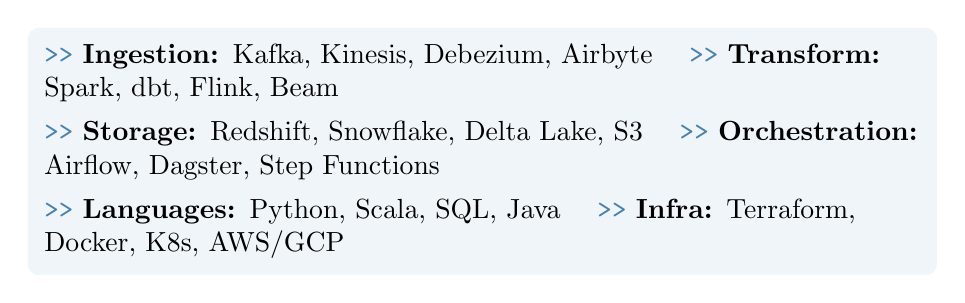
\begin{tikzpicture}
\node[fill=lightbg,rounded corners,inner sep=6pt,text width=\textwidth-1cm] {
\pipeline{\textbf{Ingestion:}} Kafka, Kinesis, Debezium, Airbyte \quad
\pipeline{\textbf{Transform:}} Spark, dbt, Flink, Beam \\[4pt]
\pipeline{\textbf{Storage:}} Redshift, Snowflake, Delta Lake, S3 \quad
\pipeline{\textbf{Orchestration:}} Airflow, Dagster, Step Functions \\[4pt]
\pipeline{\textbf{Languages:}} Python, Scala, SQL, Java \quad
\pipeline{\textbf{Infra:}} Terraform, Docker, K8s, AWS/GCP
};
\end{tikzpicture}

\section{Experience}

\noindent\textbf{Senior Data Engineer} \hfill \textcolor{accent}{Mar 2021 -- Present}\\
\textit{StreamScale Technologies, Seattle, WA}
\begin{itemize}[leftmargin=1.2em,nosep,label=\textcolor{accent}{\texttt{|>}}]
\item Architected real-time data platform processing 2M+ events/sec using Kafka and Flink
\item Migrated legacy ETL to modern ELT with dbt, reducing transformation time from 8hrs to 45min
\item Designed data mesh architecture enabling 15 domain teams to own their data products
\item Built automated data quality framework catching 95\% of anomalies before downstream impact
\end{itemize}
\vspace{0.5em}

\noindent\textbf{Data Engineer} \hfill \textcolor{accent}{Jul 2018 -- Feb 2021}\\
\textit{CloudData Corp., Portland, OR}
\begin{itemize}[leftmargin=1.2em,nosep,label=\textcolor{accent}{\texttt{|>}}]
\item Built and maintained 200+ Airflow DAGs processing 50TB daily across multiple data sources
\item Implemented CDC pipelines reducing data freshness from 24hrs to under 5 minutes
\item Optimized Redshift cluster performance, saving \$300K annually in compute costs
\end{itemize}
\vspace{0.5em}

\noindent\textbf{Junior Data Engineer} \hfill \textcolor{accent}{Jun 2017 -- Jun 2018}\\
\textit{DataFirst Analytics, San Jose, CA}
\begin{itemize}[leftmargin=1.2em,nosep,label=\textcolor{accent}{\texttt{|>}}]
\item Developed Python ETL scripts migrating on-premise data warehouse to AWS
\item Created monitoring dashboards tracking pipeline health and SLA compliance
\end{itemize}

\section{Education}
\noindent\textbf{B.S. Computer Science} \hfill University of Washington, 2017

\section{Certifications}
\noindent AWS Certified Data Analytics -- Specialty \quad\textcolor{accent}{|}\quad Databricks Certified Data Engineer \quad\textcolor{accent}{|}\quad GCP Professional Data Engineer

\end{document}
